\subsection{Direct random-streamfunction ensemble}
\label{app:random-streamfunction}
The ensemble contains 20 fixed fields per topology, indexed 0--19. The \hyperref[tab:random-historical-capacity]{numerical capacity study} and \hyperref[tab:random-paired]{learned/numerical $K=32$ allocation ablation} use this ensemble. The all-method $K=1024$ dynamic comparison uses fields 0 and 1 in each topology, with six independently qualified references. Each reported comparison uses identical physical target fields across methods and completion arms.

\subsubsection{Sampling and boundary conditioning}
We draw independent standard-normal scalar values on a $25\times25$ lattice spanning $[-1,11]\times[-6,6]$, with spacing $0.5$, and interpolate them with an exact tensor-product quintic B-spline {\citep{deboor1978splines}}. The seed hierarchy is $[20260928,\text{topology index},\text{field index}]$, with topology indices 0, 1, and 2. The spline is $C^4$ before boundary conditioning, and the final streamfunction is at least $C^2$.

Let $s$ be the raw spline and $q_j$ a smooth nonnegative defining function for boundary component $j$. The boundary indices $i,j,k$ run from $0$ to $h$. The outer component has $q_0=1-((x-5)/4)^{12}-(y/4)^{12}$; the obstacles use the original circle, rounded-square, and smoothed-triangle defining functions. For each component, $c_j$ is the arc-length-weighted mean of $s$ over 1536 boundary points. We construct bounded defining functions $\sigma_j$, partition weights $w_j$, logarithmic functions $\ell_j$, squared distance estimates $d_j^2$, and localized blending functions $b_j$. These give the boundary-adjusted field $p$, vorticity-correction weight $a$, and final streamfunction $\psi$:
\begin{align}
\sigma_j&=q_j/\sqrt{1+q_j^2},&
w_j&=\frac{\prod_{i\ne j}\sigma_i}{\sum_k\prod_{i\ne k}\sigma_i},\\
\ell_j&=\log(1+q_j),&
d_j^2&=\frac{\ell_j^2}{|\nabla\ell_j|^2+(\ell_j/4)^2+10^{-30}},\\
b_j&=w_j^3\exp\!\left[-\left(d_j^2/0.35^2\right)^2\right],&
p&=s+\sum_j b_j(c_j-s),\\
a&=\tfrac12\sum_j d_j^2b_j,&
\psi&=p-a\Delta p.
\end{align}
This construction retains a separate constant on each boundary component and enforces the original impermeability and zero-boundary-vorticity conditions. Velocity and vorticity follow from analytic derivatives, $u=(\partial_y\psi,-\partial_x\psi)$ and $\omega=-\Delta\psi$. One global scale sets the maximum sampled speed to $0.5$ on the original $321\times321$ mask and boundary loops; this scale is fixed under all numerical refinements. The distribution, raw lattice values, boundary constants, and scales define each reproducible draw; harmonic content is measured from the resulting velocity field.

\subsubsection{Captured energy, reference coordinates, and independent samples}
Assessment uses arrays of $1{,}048{,}576$, $4{,}194{,}304$, and $4{,}194{,}304$ points. Their common all-method masks contain $1{,}048{,}092$, $4{,}192{,}289$, and $4{,}192{,}265$ points. These are quadrature/assessment locations. The \hyperref[tab:random-historical-capacity]{state dimensions below} are counted from continuous piecewise-cubic (P3) reference finite-element spaces.

Using the common velocity assessment matrix $W$, let $M=U^{\top}WU$ be the mass matrix, $b=U^{\top}Wu_0$ the initial load vector, and $n=u_0^{\top}Wu_0$ the squared target norm. The full-mass initial projection gives
\begin{equation}
Mc_0=b,\qquad
\eta=\frac{c_0^{\top}Mc_0}{n}=\frac{\tfrac12\|Uc_0\|_W^2}{\tfrac12\|u_0\|_W^2}.
\end{equation}
Here $\eta$ is the fraction of initial kinetic energy represented by the projected field. Projection orthogonality gives $\eta=1-e_0^2$ for each field, where $e_0=\|Uc_0-u_0\|_W/\|u_0\|_W$. We compute the quadratic energy separately for every field and training seed before averaging. An overbar on scalar statistics denotes the ensemble mean. The mean is therefore $\overline\eta=1-\overline{e_0^2}$; no transformation of the ensemble-mean error is used. All coordinates are retained without a ridge term. Across the 840 saved $K=32$ and 120 numerical $K=1024$ projections, direct quadratic-energy and load-energy ratios agree within $1.3\times10^{-13}$.

The one-, two-, and three-hole P3 meshes have $881{,}793$, $669{,}533$, and $1{,}390{,}768$ scalar nodes. Their boundary nodes number $9{,}216$, $13{,}458$, and $22{,}428$. With constant streamfunction trace on each component and the outer constant fixed, writing $N_{\rm P3}$ for the scalar node count and $N_\partial$ for the boundary node count, the velocity-state dimension is
\begin{equation}
N_{\rm ref}=N_{\rm P3}-N_{\partial}+h.
\end{equation}
Equivalently, the reference evolves interior vorticity values and $h$ circulations; streamfunction is reconstructed from that state. This gives $N_{\rm ref}=872{,}578$, $656{,}077$, and $1{,}368{,}343$. The counts in \docref{Table}{tab:random-historical-capacity} define the state-coordinate compression ratio $N_{\rm ref}/K$, visualized in \docref{Figure}{fig:random-k1024-energy}. The same mesh dimensions apply to both reduced capacities in each domain. Initial representation checks cover all 60 P3 fields. The six predetermined fields in \docref{Appendix}{app:random-k1024-six} additionally have full-trajectory refinement measurements.

\begin{table}[!htb]\centering\small
\caption{Initial kinetic-energy capture and reference state dimensions for 20 direct random-streamfunction fields per topology. P3 nodes count the reference mesh; $N_{\rm ref}$ counts independent interior scalar coordinates plus $h$ circulations after boundary constraints and outer-gauge fixing. $K$ is the reduced state dimension, and $\eta_P,\eta_{PH}$ are mean captured-energy percentages for numerical $P_K$ and $P_{K-h}+H_h$. Energy fractions are evaluated per field before averaging. The common assessment measure, basis discretizations, and initial reference qualification are specified in \docref{Appendix}{app:random-streamfunction}.}
\label{tab:random-historical-capacity}
\setlength{\tabcolsep}{4pt}
\begin{tabular}{rrrrrr}\toprule
Holes & P3 nodes & $N_{\rm ref}$ & $K$ & $\eta_P$ (\%) & $\eta_{PH}$ (\%)\\\midrule
1&881,793&872,578&32&2.27&2.13\\
1&881,793&872,578&1024&75.32&75.34\\
2&669,533&656,077&32&2.37&2.16\\
2&669,533&656,077&1024&79.66&79.73\\
3&1,390,768&1,368,343&32&1.79&1.60\\
3&1,390,768&1,368,343&1024&54.48&54.52\\
\bottomrule\end{tabular}\end{table}

\subsubsection{Optional combined energy--compression summary}
\label{app:basis-quality}
For a fixed reference discretization, captured energy and compression in \docref{Figure}{fig:random-k1024-energy} define the energy--compression product $Q_B$. Let $E_{\rm projected}$ and $E_{\rm target}$ denote initial projected and target kinetic energies; then
\begin{equation}
Q_B=\eta\frac{N_{\rm ref}}{K}
=\frac{E_{\rm projected}/K}{E_{\rm target}/N_{\rm ref}}.
\label{eq:basis-energy-quality}
\end{equation}
For field $i$, $Q_{B,i}=(N_{\rm ref}/K)\eta_i$, so $\overline Q_B=(N_{\rm ref}/K)\overline\eta$. This is a derived summary of energy capture and compression. At fixed $N_{\rm ref}$ and $K$ it orders methods exactly as $\eta$ does. Its reference normalization changes under mesh refinement. We therefore report the independently interpretable energy fractions and compression ratios in the \hyperref[fig:random-k1024-energy]{main text}, and retain the \hyperref[tab:basis-quality]{combined values here} for a common reference convention.
\begin{table}[!htb]\centering\small
\caption{Derived energy--compression products for the numerical representations in \docref{Table}{tab:random-historical-capacity}. Energy fractions are evaluated per field before averaging; all 20 draws per topology are retained.}
\label{tab:basis-quality}
\begin{tabular}{rrrr}\toprule
Holes&$K$&$\overline Q_{B,P}$&$\overline Q_{B,PH}$\\\midrule
1&32&618.62&581.29\\
1&1024&641.84&641.99\\
2&32&485.62&442.04\\
2&1024&510.41&510.82\\
3&32&767.13&685.73\\
3&1024&728.05&728.60\\
\bottomrule\end{tabular}\end{table}

The $K=32$ bases use their original common P1 embeddings. The numerical $K=1024$ bases use their original level-2 P1 representations. Both are assessed against the same continuous analytic initial fields on the unchanged common masks. The capacity table compares these existing discretized representations; their basis meshes differ. All 20 fields are retained at each capacity.

The Laplacian basis contributes one numerical realization; potential and velocity training each contribute three existing seeds at $K=32$. For each learned method, captured-energy fractions are averaged across seeds within a field, then over the 20 independent fields. \docref{Table}{tab:random-paired} reports mean capture and the paired gain $\Delta\eta=\eta_{PH}-\eta_P$ in percentage points. This equal-total-$K$ comparison exchanges $h$ positive coordinates for $h$ harmonic coordinates.

\begin{table}[!htb]\centering\small
\caption{Initial kinetic-energy capture at total $K=32$, in percent. $\Delta\eta$ is the mean captured-energy change in percentage points. Positive values favor completion. Learned energy fractions average three seeds within each of the 20 independent fields; the last column counts fields with higher $PH$ capture.}
\label{tab:random-paired}
\begin{tabular}{rlrrrr}\toprule
Holes & Basis & $\eta_P$ (\%) & $\eta_{PH}$ (\%) & $\Delta\eta$ & Improved\\\midrule
1&Laplacian&2.269&2.132&-0.137&2/20\\
1&Potential&2.252&2.178&-0.075&5/20\\
1&Velocity&2.269&2.145&-0.124&2/20\\
2&Laplacian&2.369&2.156&-0.213&3/20\\
2&Potential&2.370&2.174&-0.197&3/20\\
2&Velocity&2.345&2.216&-0.129&3/20\\
3&Laplacian&1.794&1.604&-0.190&3/20\\
3&Potential&1.795&1.633&-0.163&2/20\\
3&Velocity&2.009&1.814&-0.195&2/20\\
\bottomrule\end{tabular}\end{table}




\begin{samepage}
\paragraph{Harmonic-energy diagnostic.}
\begingroup
The 60 directly sampled fields predominantly occupy the vortical sector. Projection onto the numerical harmonic span gives median initial energy fractions of $0.01016\%$, $0.06411\%$, and $0.04385\%$ for one, two, and three holes, with maxima of $0.11744\%$, $0.17651\%$, and $0.27178\%$. Level-2/level-3 harmonic refinement changes these fractions by at most $0.00214$ percentage points. At fixed $K$, mass-orthogonal sectors trade the harmonic projection energy gained against the energy of the $h$ displaced positive modes. The coordinate allocation is therefore governed by the relative occupation of these two sectors. Positive modes are ordered by spectral Rayleigh values; a field's captured energy depends on its modal coefficients. Appending $H_h$ to unchanged $P_K$ creates a nested span, whose best-projection error is nonincreasing.
\par\endgroup
\par
\end{samepage}

\subsubsection{Autonomous trajectories for the first one- and two-hole draws}
\label{app:random-dynamics}
The $K=32$ comparison uses the first fixed draw (index 0) in each of the one- and two-hole domains. Each method starts from the analytic-field full-mass projection and evolves autonomously with the reused Galerkin operators, $\nu=1/750$, $T=1$, and 51 saved frames. The two step sizes are $0.002$ and $0.001$. Subsequent reference values enter error assessment, not the coefficient evolution. \docref{Table}{tab:random-dynamics} summarizes the fine-step errors. {With $\bar e=\int_0^1e(t)\,\dd t$ the time-averaged relative error, we define the improvement $\Delta(t)=e_P(t)-e_{PH}(t)$ and $\bar\Delta=\bar e_P-\bar e_{PH}$; positive values mean lower error after completion.}

The numerical reference uses continuous cubic finite elements and the fine time step. Maximum coarse/fine relative velocity differences are $2.53042\times10^{-6}$ and $5.03966\times10^{-5}$. Full-trajectory quadratic/cubic comparisons give $0.84444\%$ and $0.72543\%$ differences; independent boundary-geometry refinement gives $0.02050\%$ and $0.07681\%$ across all 51 frames on both original masks. These checks retain the same analytic initial field. Direct-field and moment-based error evaluation agree to below $6.10\times10^{-16}$; the independent polynomial point-adapter check is below $3.33\times10^{-13}$. This table reports the two $K=32$ dynamic cases; the \hyperref[app:random-k1024-six]{complete six-field $K=1024$ assessment} is reported next.

\begin{table}[!htb]\centering\small
\caption{Random-field dynamics for index 0 in each of two domains. $\bar e=\int_0^1e_u(t)\,\mathrm dt$ is evaluated by the trapezoidal rule over 51 frames. Errors are percentages and differences are percentage points. Learned entries average the three training seeds of the same physical field.}
\label{tab:random-dynamics}
\begin{tabular}{rlrrrr}\toprule
Holes&Basis&$\bar e_P$&$\bar e_{PH}$&$\bar\Delta$&$\Delta(T)$\\\midrule
1&Laplacian&99.28325&99.29712&-0.01387&-0.01336\\
1&Potential&99.26077&99.26889&-0.00812&-0.00733\\
1&Velocity&99.27255&99.29087&-0.01832&-0.01817\\
2&Laplacian&98.75970&98.79192&-0.03221&-0.02997\\
2&Potential&98.79390&98.84504&-0.05114&-0.05093\\
2&Velocity&98.81309&98.91302&-0.09993&-0.10682\\
\bottomrule\end{tabular}\end{table}



\subsubsection{Six-field \texorpdfstring{$K=1024$}{K=1024} comparison}
\label{app:random-k1024-six}
All methods use the fixed indices 0 and 1, full-rank mass projection of the analytic initial field, and all 1024 coordinates. Existing learned checkpoints, numerical operators, and NKB models are reused. Reduced trajectories were advanced as 20-field batches; this assessment selects the two predetermined fields without changing their coefficients. Coarse/fine steps are $0.002/0.001$ with 51 saved frames on $[0,1]$ and $\nu=1/750$. No later reference state enters autonomous integration. Initial-energy fractions use the assessment mass, which is distinct from the operator quadrature mass.

Reference refinement tests compare the same physical fields under time-step, polynomial-space, and boundary-geometry changes on both original masks. For the three-hole fields, the largest time-step differences are $0.02414\%$ and $0.03835\%$; polynomial-space differences are $0.49879\%$ and $0.92725\%$; geometry differences are $0.10612\%$ and $0.17219\%$. The initial physical fields and evaluation masks remain fixed under all refinements. The reported relative velocity errors use the original common all-method masks; analytic-only supplementary points are reported separately where the representation is defined.

\docref{Figure}{fig:random-k1024-energy} gives initial capture and compression, and \docref{Figure}{fig:random-k1024-errors} shows all autonomous error curves. The paired allocation gains are reported in \docref{Table}{tab:completion-improvement}.

\begin{figure}[!htb]\centering
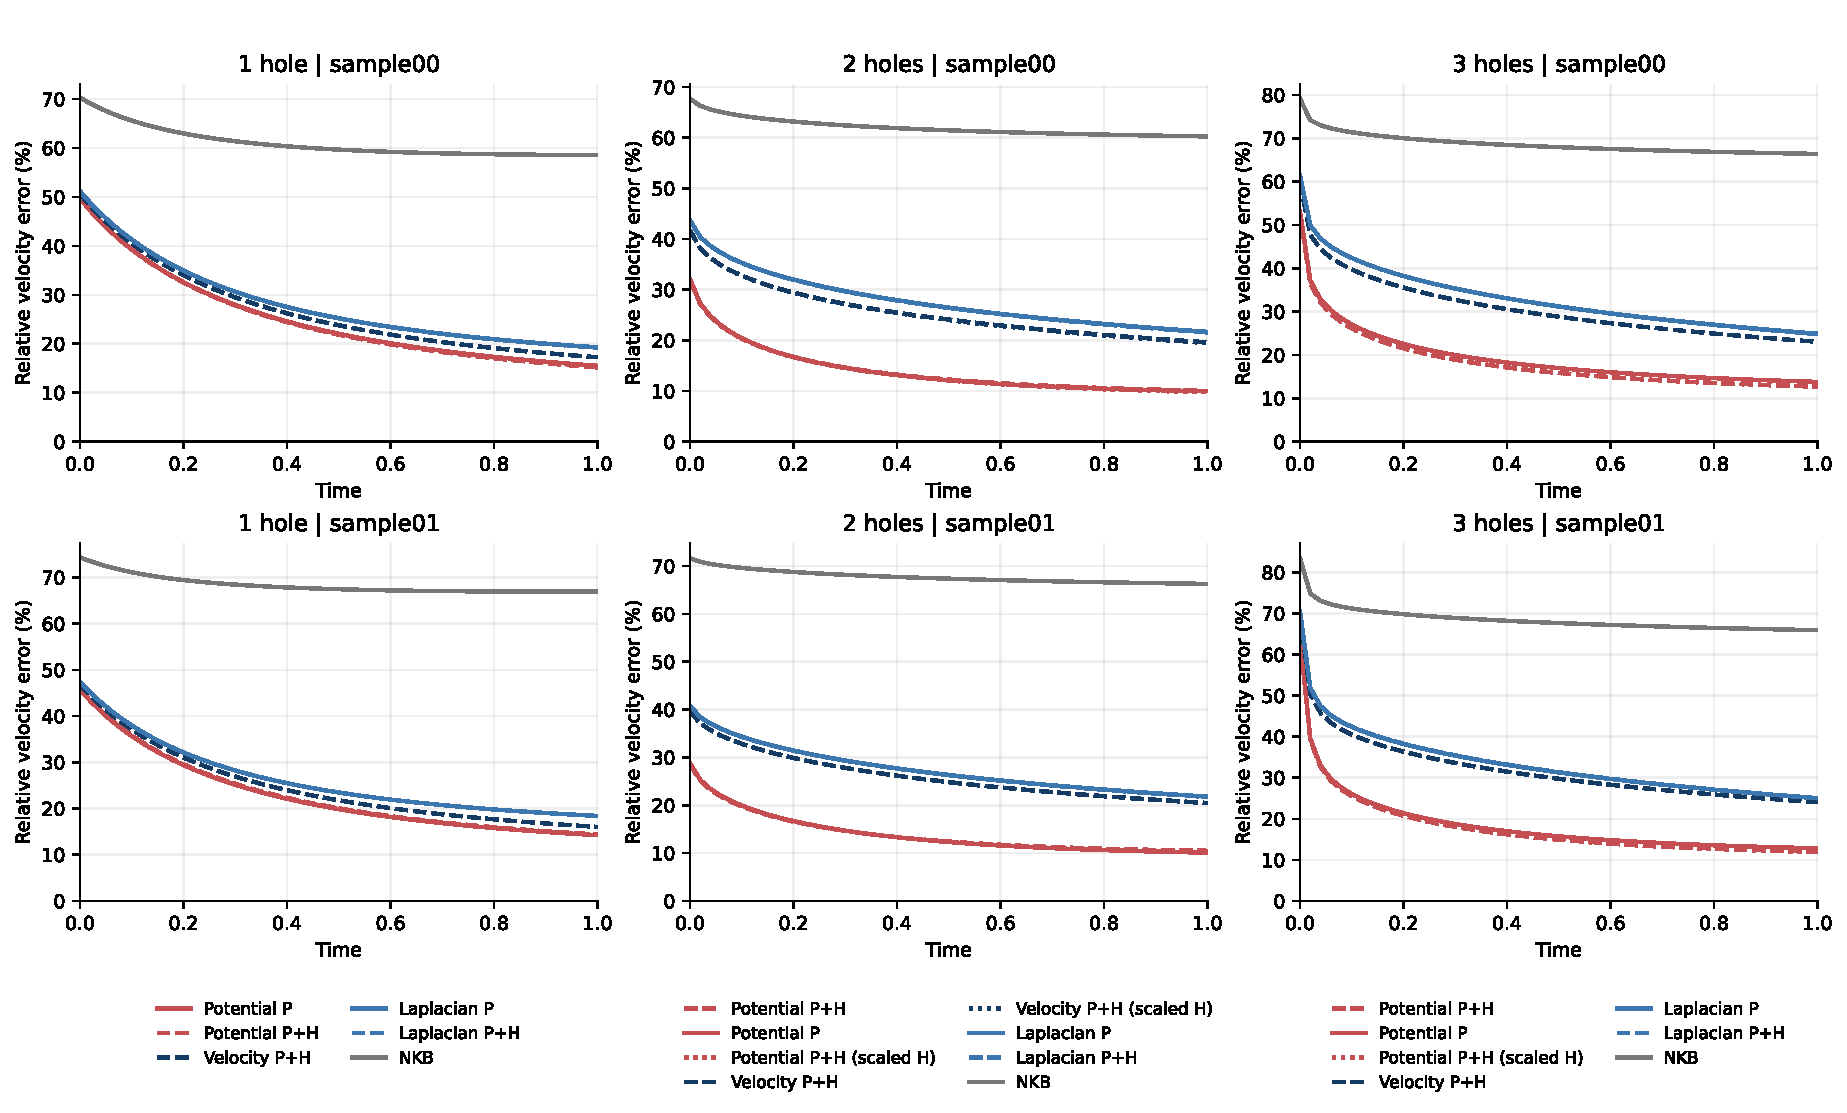
\includegraphics[width=\linewidth,height=.72\textheight,keepaspectratio]{unified_names_20261021_v1/random_k1024_final_velocity_errors.pdf}
\caption{All six autonomous random-field comparisons at $K=1024$ against qualified references. Each panel is one predetermined physical field, and every curve uses all 51 saved times and the original common mask. The numerical control has the same total coordinate count and the corresponding P or P+H allocation.}
\label{fig:random-k1024-errors}
\end{figure}

For a saved coefficient vector, let $M_{\rm assessment}=U^{\top}WU$ denote the full mass matrix on assessment nodes. Its quadratic energy is $c^{\top}M_{\rm assessment}c$ (twice the kinetic energy). Explicit harmonic components are reported both through their own coefficients and as the mass-orthogonal projection of the full velocity onto each method's harmonic span. Let $H$ index the harmonic coordinates, $M_{HH}$ be their mass block, and $\ell_H$ the harmonic entries of the full velocity load. The latter quadratic energy is $\ell_H^{\top}M_{HH}^{-1}\ell_H$, with $\ell_H=(M_{\rm assessment}c)_H$, retaining P/H cross terms. Learned harmonic fields use their original learned representation throughout.

\begin{figure}[htbp]\centering
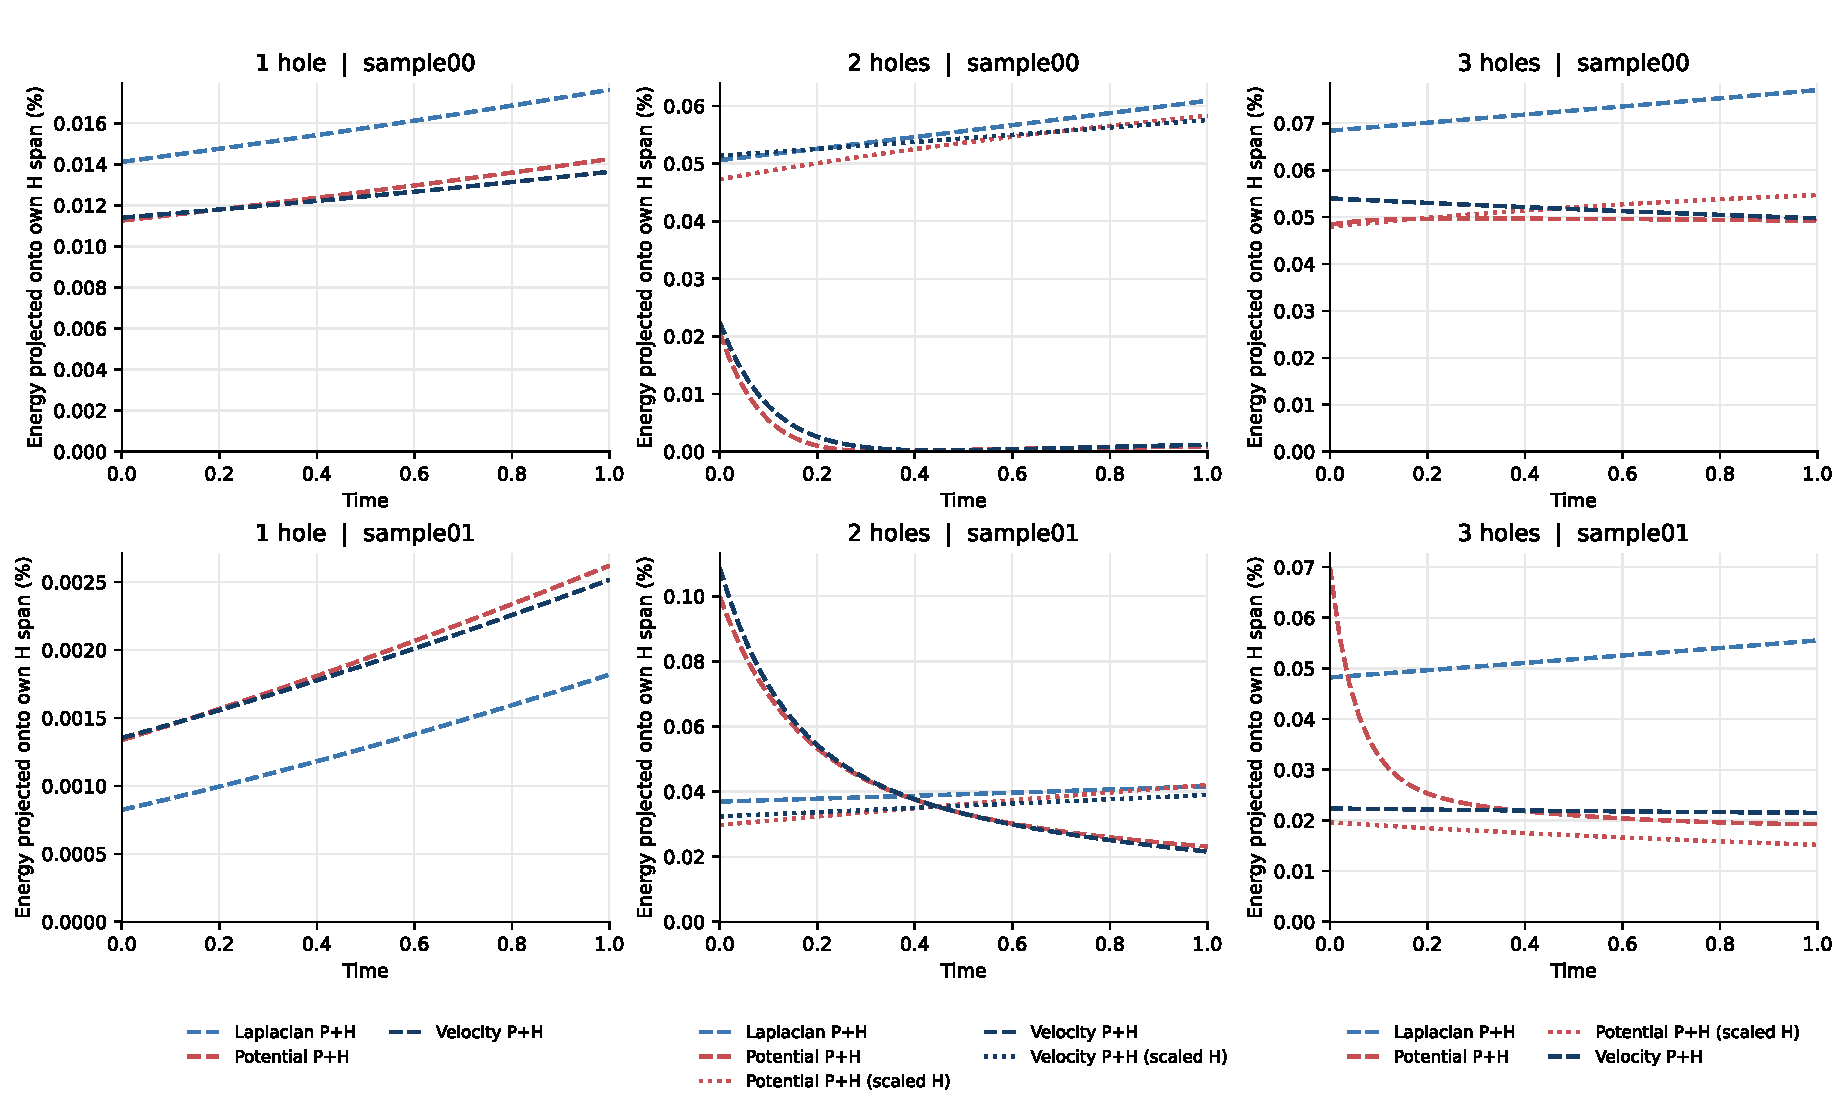
\includegraphics[width=\linewidth,height=.72\textheight,keepaspectratio]{unified_names_20261021_v1/random_k1024_trajectory_harmonic_fraction.pdf}
\caption{Energy projected onto each representation's explicit harmonic span as a fraction of its instantaneous total energy. The projection measures occupation of each representation's explicit circulation coordinates.}
\label{fig:random-k1024-harmonic}
\end{figure}

Supplementary boundary diagnostics use exact edge integration of the original P1 polygon velocities for numerical bases, and nested 1024/2048-point analytic-boundary evaluations for neural bases. They report normal speed and counterclockwise circulation around each enclosed component over all 51 frames. Curl-form neural velocities have cancelling analytic mixed derivatives; NKB divergence is evaluated from its analytic direct-velocity Jacobian at 1024 deterministic original common-mask points. These component diagnostics complement the full-domain error measurements. The released results include all per-component circulation curves, quadrature-refinement differences, and energy histories.

The timing ledger separates reference generation and qualification, cache/operator recovery, projection, batched evolution, and error assessment. Existing 20-field batch costs remain associated with those batches. Stage and process timers retain their respective workload boundaries. Supplementary boundary diagnostics required 390.59 seconds across their measured stages, independently of reference generation and final full-domain error assessment.

